\renewcommand{\NomeBloco}{\emph{NAND}}
\renewcommand{\NomeBlocoNoIt}{NAND}
\renewcommand{\NomePTab}{tab_\NomeBlocoNoIt}
\renewcommand{\NomeSTab}{tab_\NomeBlocoNoIt2}
\renewcommand{\NomePFig}{fig_\NomeBlocoNoIt}
\renewcommand{\NomeSFig}{fig_\NomeBlocoNoIt2}
\renewcommand{\NomeTTab}{tab_\NomeBlocoNoIt3}

\section{NAND}

O bloco \NomeBloco{} tem a finalidade de receber duas entradas digitais, e rcolocar o resultado da opera ção NAND em sua sa\'ida. A \autoref{\NomePTab} indica a Tabela Verdade do bloco.

\begin{table}[htbp]

\caption{Tabela Verdade do bloco \NomeBloco}%
\label{\NomePTab}
\centering
\begin{tabular}{ccc}
\toprule
    A & B & Out \\
    \midrule \midrule
    0 & 0 & 1 \\
    \midrule
    0 & 1 & 1\\
    \midrule
    1 & 0 & 1\\
    \midrule
    1 & 1 & 0\\
\bottomrule

\end{tabular}
\fonte{Produzido pelo autor.}
\end{table}

O bloco apresenta as defini ções de sinais de entrada e sa\'ida referidos na \autoref{\NomeSTab}.

\begin{table}[htbp]
\caption{Sinais do bloco \NomeBloco}
\label{\NomeSTab}
\centering
\begin{tabular}{ccl}

    \toprule
    Sinal & Tipo    & Descri ção        \\
    \midrule \midrule
    A    & Entrada & Sinal de Entrada A \\
    \midrule
    B    & Entrada & Sinal de Entrada B \\
    \midrule
    Out    & Sa\'ida & Sinal de sa\'ida \\
    \bottomrule
\end{tabular}
\legend{Fonte: Produzido pelo autor}
\end{table}

O circuito projetado para o bloco \'e demonstrado na \autoref{\NomePFig}.

\begin{figure}[htbp]
 \label{NomePFig}
 \centering
  \begin{minipage}{0.4\textwidth}
    \centering
    \caption{Circuito CMOS projetado para o bloco \NomeBloco} \label{\NomePFig}
    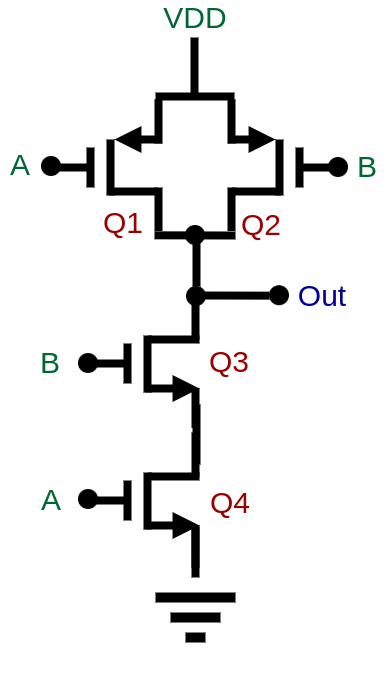
\includegraphics[scale=0.3]{Circuitos/NAND.png}
    \legend{Fonte: Produzido pelo autor}
  \end{minipage}
  \hfill
  \begin{minipage}{0.4\textwidth}
    \centering
    \caption{Representa ção em bloco do \NomeBlocoNoIt} \label{NomeSFig}
    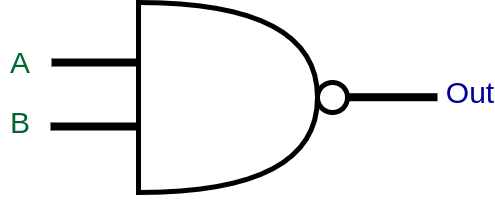
\includegraphics[scale=0.3]{Circuitos/NAND_block.png}
    \legend{Fonte: Produzido pelo autor}
  \end{minipage}
\end{figure}